\documentclass[11pt,]{article}
\usepackage{lmodern}
\usepackage{amssymb,amsmath}
\usepackage{ifxetex,ifluatex}
\usepackage{fixltx2e} % provides \textsubscript
\ifnum 0\ifxetex 1\fi\ifluatex 1\fi=0 % if pdftex
  \usepackage[T1]{fontenc}
  \usepackage[utf8]{inputenc}
\else % if luatex or xelatex
  \ifxetex
    \usepackage{mathspec}
    \usepackage{xltxtra,xunicode}
  \else
    \usepackage{fontspec}
  \fi
  \defaultfontfeatures{Mapping=tex-text,Scale=MatchLowercase}
  \newcommand{\euro}{€}
\fi
% use upquote if available, for straight quotes in verbatim environments
\IfFileExists{upquote.sty}{\usepackage{upquote}}{}
% use microtype if available
\IfFileExists{microtype.sty}{%
\usepackage{microtype}
\UseMicrotypeSet[protrusion]{basicmath} % disable protrusion for tt fonts
}{}
\usepackage[margin=1in]{geometry}
\usepackage{color}
\usepackage{fancyvrb}
\newcommand{\VerbBar}{|}
\newcommand{\VERB}{\Verb[commandchars=\\\{\}]}
\DefineVerbatimEnvironment{Highlighting}{Verbatim}{commandchars=\\\{\}}
% Add ',fontsize=\small' for more characters per line
\usepackage{framed}
\definecolor{shadecolor}{RGB}{248,248,248}
\newenvironment{Shaded}{\begin{snugshade}}{\end{snugshade}}
\newcommand{\KeywordTok}[1]{\textcolor[rgb]{0.13,0.29,0.53}{\textbf{{#1}}}}
\newcommand{\DataTypeTok}[1]{\textcolor[rgb]{0.13,0.29,0.53}{{#1}}}
\newcommand{\DecValTok}[1]{\textcolor[rgb]{0.00,0.00,0.81}{{#1}}}
\newcommand{\BaseNTok}[1]{\textcolor[rgb]{0.00,0.00,0.81}{{#1}}}
\newcommand{\FloatTok}[1]{\textcolor[rgb]{0.00,0.00,0.81}{{#1}}}
\newcommand{\CharTok}[1]{\textcolor[rgb]{0.31,0.60,0.02}{{#1}}}
\newcommand{\StringTok}[1]{\textcolor[rgb]{0.31,0.60,0.02}{{#1}}}
\newcommand{\CommentTok}[1]{\textcolor[rgb]{0.56,0.35,0.01}{\textit{{#1}}}}
\newcommand{\OtherTok}[1]{\textcolor[rgb]{0.56,0.35,0.01}{{#1}}}
\newcommand{\AlertTok}[1]{\textcolor[rgb]{0.94,0.16,0.16}{{#1}}}
\newcommand{\FunctionTok}[1]{\textcolor[rgb]{0.00,0.00,0.00}{{#1}}}
\newcommand{\RegionMarkerTok}[1]{{#1}}
\newcommand{\ErrorTok}[1]{\textbf{{#1}}}
\newcommand{\NormalTok}[1]{{#1}}
\usepackage{graphicx}
\makeatletter
\def\maxwidth{\ifdim\Gin@nat@width>\linewidth\linewidth\else\Gin@nat@width\fi}
\def\maxheight{\ifdim\Gin@nat@height>\textheight\textheight\else\Gin@nat@height\fi}
\makeatother
% Scale images if necessary, so that they will not overflow the page
% margins by default, and it is still possible to overwrite the defaults
% using explicit options in \includegraphics[width, height, ...]{}
\setkeys{Gin}{width=\maxwidth,height=\maxheight,keepaspectratio}
\ifxetex
  \usepackage[setpagesize=false, % page size defined by xetex
              unicode=false, % unicode breaks when used with xetex
              xetex]{hyperref}
\else
  \usepackage[unicode=true]{hyperref}
\fi
\hypersetup{breaklinks=true,
            bookmarks=true,
            pdfauthor={David J. Harris},
            pdftitle={Appendix 3: Estimating species interactions},
            colorlinks=true,
            citecolor=blue,
            urlcolor=blue,
            linkcolor=magenta,
            pdfborder={0 0 0}}
\urlstyle{same}  % don't use monospace font for urls
\setlength{\parindent}{0pt}
\setlength{\parskip}{6pt plus 2pt minus 1pt}
\setlength{\emergencystretch}{3em}  % prevent overfull lines
\setcounter{secnumdepth}{0}

%%% Use protect on footnotes to avoid problems with footnotes in titles
\let\rmarkdownfootnote\footnote%
\def\footnote{\protect\rmarkdownfootnote}

%%% Change title format to be more compact
\usepackage{titling}

% Create subtitle command for use in maketitle
\newcommand{\subtitle}[1]{
  \posttitle{
    \begin{center}\large#1\end{center}
    }
}

\setlength{\droptitle}{-2em}
  \title{Appendix 3: Estimating species interactions}
  \pretitle{\vspace{\droptitle}\centering\huge}
  \posttitle{\par}
\subtitle{"Estimating species interactions from observational data with Markov
networks"}
  \author{David J. Harris}
  \preauthor{\centering\large\emph}
  \postauthor{\par}
  \date{}
  \predate{}\postdate{}



\begin{document}

\maketitle


This document describes how the different models were fit to the
simulated data from Appendix 2 and how each model's performance was
evaluated.\footnote{The PDF version of this document has been manually
  altered to omit 150 lines of output from the \texttt{corpcor} package
  of the form
  ``\texttt{\#\#\ Estimating\ optimal\ shrinkage\ intensity\ lambda\ (correlation\ matrix):\ 0.0326}''}

Initialization:

\begin{Shaded}
\begin{Highlighting}[]
\KeywordTok{library}\NormalTok{(dplyr)        }\CommentTok{# For manipulating data structures}
\KeywordTok{library}\NormalTok{(corpcor)      }\CommentTok{# For regularized partial covariances}
\KeywordTok{library}\NormalTok{(rosalia)      }\CommentTok{# For Markov networks}
\KeywordTok{library}\NormalTok{(arm)          }\CommentTok{# For regularized logistic regression}
\KeywordTok{library}\NormalTok{(BayesComm)    }\CommentTok{# For joint species distribution modeling}
\KeywordTok{library}\NormalTok{(RColorBrewer) }\CommentTok{# For color palette}
\KeywordTok{set.seed}\NormalTok{(}\DecValTok{1}\NormalTok{)}
\end{Highlighting}
\end{Shaded}

Load in the results from the \texttt{pairs} program, run outside of R
with the following options:

\begin{itemize}
\itemsep1pt\parskip0pt\parsep0pt
\item
  Batch mode
\item
  Sequential swap (``s'')
\item
  Printing all pairs (``y'')
\item
  C-score co-occurrence measure (``c'')
\item
  Default confidence limits (0.05)
\item
  Default iterations (100)
\item
  Maximum of 20 species
\end{itemize}

\begin{Shaded}
\begin{Highlighting}[]
\NormalTok{pairs_txt =}\StringTok{ }\KeywordTok{readLines}\NormalTok{(}\StringTok{"fakedata/Pairs.txt"}\NormalTok{)}

\CommentTok{# Find areas of the data file that correspond}
\CommentTok{# to species pairs' results}
\NormalTok{beginnings =}\StringTok{ }\KeywordTok{grep}\NormalTok{(}\StringTok{"Sp1"}\NormalTok{, pairs_txt) +}\StringTok{ }\DecValTok{1}
\NormalTok{ends =}\StringTok{ }\KeywordTok{c}\NormalTok{(}
  \KeywordTok{grep}\NormalTok{(}\StringTok{"^[^ ]"}\NormalTok{, pairs_txt)[-}\DecValTok{1}\NormalTok{],}
  \KeywordTok{length}\NormalTok{(pairs_txt)}
\NormalTok{) -}\StringTok{ }\DecValTok{1}

\CommentTok{# The above code fails on the very last line of the file}
\NormalTok{ends[}\KeywordTok{length}\NormalTok{(ends)] =}\StringTok{ }\NormalTok{ends[}\KeywordTok{length}\NormalTok{(ends)] +}\StringTok{ }\DecValTok{1}
\end{Highlighting}
\end{Shaded}

A function to import the data file and run each method on it:

\begin{Shaded}
\begin{Highlighting}[]
\NormalTok{fit_all =}\StringTok{ }\NormalTok{function(filename)\{}
  \NormalTok{######## Import ########}
  
  \CommentTok{# Multiplying by one is necessary to prevent silly errors}
  \CommentTok{# regarding TRUE/FALSE versus 1/0}
  \NormalTok{raw_obs =}\StringTok{ }\KeywordTok{readRDS}\NormalTok{(filename)[[}\StringTok{"observed"}\NormalTok{]] *}\StringTok{ }\DecValTok{1}
  
  \CommentTok{# Identify species that are never present (or never absent) so they }
  \CommentTok{# can be dropped}
  \NormalTok{species_is_variable =}\StringTok{ }\KeywordTok{diag}\NormalTok{(}\KeywordTok{var}\NormalTok{(raw_obs)) >}\StringTok{ }\DecValTok{0}
  \NormalTok{pair_is_variable =}\StringTok{ }\KeywordTok{tcrossprod}\NormalTok{(species_is_variable) >}\StringTok{ }\DecValTok{0}
  
  \NormalTok{x =}\StringTok{ }\NormalTok{raw_obs[ , species_is_variable]}
  \NormalTok{truth =}\StringTok{ }\KeywordTok{readRDS}\NormalTok{(filename)[[}\StringTok{"truth"}\NormalTok{]][pair_is_variable[}\KeywordTok{upper.tri}\NormalTok{(pair_is_variable)]]}
  
  \NormalTok{splitname =}\StringTok{ }\KeywordTok{strsplit}\NormalTok{(filename, }\StringTok{"/|-|}\CharTok{\textbackslash{}\textbackslash{}}\StringTok{."}\NormalTok{)[[}\DecValTok{1}\NormalTok{]]}
  \NormalTok{n_sites =}\StringTok{ }\KeywordTok{as.integer}\NormalTok{(splitname[[}\DecValTok{3}\NormalTok{]])}
  \NormalTok{rep =}\StringTok{ }\KeywordTok{as.integer}\NormalTok{(splitname[[}\DecValTok{4}\NormalTok{]])}
  
  
  \NormalTok{######## Partial correlations ########}
  \NormalTok{p_corr =}\StringTok{ }\KeywordTok{pcor.shrink}\NormalTok{(x)}
  
  \NormalTok{######## Correlations ########}
  \NormalTok{corr =}\StringTok{ }\KeywordTok{cor}\NormalTok{(x)}
  
  \NormalTok{######## GLM ########}
  \NormalTok{coef_matrix =}\StringTok{ }\KeywordTok{matrix}\NormalTok{(}\DecValTok{0}\NormalTok{, }\KeywordTok{ncol}\NormalTok{(x), }\KeywordTok{ncol}\NormalTok{(x))}
  \NormalTok{for(i in }\DecValTok{1}\NormalTok{:}\KeywordTok{ncol}\NormalTok{(x))\{}
    \NormalTok{if(}\KeywordTok{var}\NormalTok{(x[,i]) >}\StringTok{ }\DecValTok{0}\NormalTok{)\{}
      \NormalTok{coefs =}\StringTok{ }\KeywordTok{coef}\NormalTok{(}\KeywordTok{bayesglm}\NormalTok{(x[,i] ~}\StringTok{ }\NormalTok{x[ , -i], }\DataTypeTok{family =} \NormalTok{binomial))[-}\DecValTok{1}\NormalTok{]}
      \NormalTok{coef_matrix[i, -i] =}\StringTok{ }\NormalTok{coefs}
    \NormalTok{\}}
  \NormalTok{\}}
  \NormalTok{coef_matrix =}\StringTok{ }\NormalTok{(coef_matrix +}\StringTok{ }\KeywordTok{t}\NormalTok{(coef_matrix)) /}\StringTok{ }\DecValTok{2}
  
  \NormalTok{######## Markov network ########}
  \NormalTok{rosie =}\StringTok{ }\KeywordTok{rosalia}\NormalTok{(x, }\DataTypeTok{maxit =} \DecValTok{200}\NormalTok{, }\DataTypeTok{trace =} \DecValTok{0}\NormalTok{, }\DataTypeTok{prior =} \KeywordTok{make_logistic_prior}\NormalTok{(}\DataTypeTok{scale =} \DecValTok{2}\NormalTok{))}
  
  \NormalTok{######## BayesComm and partial BayesComm ########}
  \NormalTok{bc =}\StringTok{ }\KeywordTok{BC}\NormalTok{(}\DataTypeTok{Y =} \NormalTok{x, }\DataTypeTok{model =} \StringTok{"community"}\NormalTok{, }\DataTypeTok{its =} \DecValTok{1000}\NormalTok{)}
  
  \StringTok{`}\DataTypeTok{partial BayesComm}\StringTok{`} \NormalTok{=}\StringTok{ }\DecValTok{0}
  
  \NormalTok{for(i in }\DecValTok{1}\NormalTok{:}\KeywordTok{nrow}\NormalTok{(bc$trace$R))\{}
    \NormalTok{Sigma =}\StringTok{ }\KeywordTok{matrix}\NormalTok{(}\DecValTok{0}\NormalTok{, }\DataTypeTok{nrow =} \KeywordTok{ncol}\NormalTok{(x), }\DataTypeTok{ncol =} \KeywordTok{ncol}\NormalTok{(x))}
    \NormalTok{Sigma[}\KeywordTok{upper.tri}\NormalTok{(Sigma)] <-}\StringTok{ }\NormalTok{bc$trace$R[i, ]  }\CommentTok{# Fill in upper triangle}
    \NormalTok{Sigma <-}\StringTok{ }\NormalTok{Sigma +}\StringTok{ }\KeywordTok{t}\NormalTok{(Sigma)                   }\CommentTok{# Fill in lower triangle}
    \KeywordTok{diag}\NormalTok{(Sigma) <-}\StringTok{ }\DecValTok{1}  \CommentTok{# Diagonal equals 1 in multivariate probit model}
    
    \StringTok{`}\DataTypeTok{partial BayesComm}\StringTok{`} \NormalTok{=}\StringTok{ `}\DataTypeTok{partial BayesComm}\StringTok{`} \NormalTok{+}\StringTok{ }\KeywordTok{cor2pcor}\NormalTok{(Sigma) /}\StringTok{ }\KeywordTok{nrow}\NormalTok{(bc$trace$R)}
  \NormalTok{\}}
  
  \NormalTok{######## Pairs ########}
  \CommentTok{# Find the line where the current data set is mentioned in}
  \CommentTok{# pairs.txt}
  \NormalTok{filename_line =}\StringTok{ }\KeywordTok{grep}\NormalTok{(}
    \KeywordTok{paste0}\NormalTok{(}
      \KeywordTok{gsub}\NormalTok{(}\StringTok{"fakedata/(.*)}\CharTok{\textbackslash{}\textbackslash{}}\StringTok{.rds"}\NormalTok{, }\StringTok{"}\CharTok{\textbackslash{}\textbackslash{}}\StringTok{1"}\NormalTok{, filename),}
      \StringTok{"-"}
    \NormalTok{),}
    \NormalTok{pairs_txt}
  \NormalTok{)}
  
  \CommentTok{# Which chunk of the data file corresponds to this file?}
  \NormalTok{chunk =}\StringTok{ }\KeywordTok{min}\NormalTok{(}\KeywordTok{which}\NormalTok{(beginnings >}\StringTok{ }\NormalTok{filename_line))}
  
  \CommentTok{# Split the chunk on whitespace.}
  \NormalTok{splitted =}\StringTok{ }\KeywordTok{strsplit}\NormalTok{(pairs_txt[beginnings[chunk]:ends[chunk]], }\StringTok{" +"}\NormalTok{)}
  
  \CommentTok{# Pull out the species numbers and their Z-scores}
  \NormalTok{pairs_results =}\StringTok{ }\KeywordTok{lapply}\NormalTok{(}
    \NormalTok{splitted,}
    \NormalTok{function(x)\{}
      \NormalTok{spp =}\StringTok{ }\KeywordTok{sort}\NormalTok{(}\KeywordTok{as.integer}\NormalTok{(x[}\DecValTok{3}\NormalTok{:}\DecValTok{4}\NormalTok{]))}
      \KeywordTok{data.frame}\NormalTok{(}
        \DataTypeTok{sp1 =} \NormalTok{spp[}\DecValTok{1}\NormalTok{], }
        \DataTypeTok{sp2 =} \NormalTok{spp[}\DecValTok{2}\NormalTok{], }
        \DataTypeTok{z =} \KeywordTok{as.numeric}\NormalTok{(x[}\DecValTok{14}\NormalTok{])}
      \NormalTok{)}
    \NormalTok{\}}
  \NormalTok{) %>%}\StringTok{ }
\StringTok{    }\NormalTok{bind_rows %>%}
\StringTok{    }\KeywordTok{mutate}\NormalTok{(}\DataTypeTok{spp =} \KeywordTok{paste}\NormalTok{(sp1, sp2, }\DataTypeTok{sep =} \StringTok{"-"}\NormalTok{))}
  
  \CommentTok{# Re-order the pairs_results to match the other methods}
  \NormalTok{m =}\StringTok{ }\KeywordTok{matrix}\NormalTok{(}\OtherTok{NA}\NormalTok{, }\KeywordTok{ncol}\NormalTok{(x), }\KeywordTok{ncol}\NormalTok{(x))}
  \NormalTok{new_order =}\StringTok{ }\KeywordTok{match}\NormalTok{(}
    \KeywordTok{paste}\NormalTok{(}\KeywordTok{row}\NormalTok{(m)[}\KeywordTok{upper.tri}\NormalTok{(m)], }\KeywordTok{col}\NormalTok{(m)[}\KeywordTok{upper.tri}\NormalTok{(m)], }\DataTypeTok{sep =} \StringTok{"-"}\NormalTok{),}
    \NormalTok{pairs_results$spp}
  \NormalTok{)}
  \NormalTok{ordered_pairs_results =}\StringTok{ }\NormalTok{pairs_results[new_order, ]}
  
  \NormalTok{######## Output ########}
  \KeywordTok{data.frame}\NormalTok{(}
    \DataTypeTok{truth =} \NormalTok{truth, }
    \DataTypeTok{n_sites =} \NormalTok{n_sites,}
    \DataTypeTok{rep =} \NormalTok{rep,}
    \DataTypeTok{sp1 =} \NormalTok{ordered_pairs_results$sp1,}
    \DataTypeTok{sp2 =} \NormalTok{ordered_pairs_results$sp2,}
    \StringTok{`}\DataTypeTok{partial correlation}\StringTok{`} \NormalTok{=}\StringTok{ }\NormalTok{p_corr[}\KeywordTok{upper.tri}\NormalTok{(p_corr)],}
    \DataTypeTok{correlation =} \NormalTok{corr[}\KeywordTok{upper.tri}\NormalTok{(corr)],}
    \StringTok{`}\DataTypeTok{Markov network}\StringTok{`} \NormalTok{=}\StringTok{ }\NormalTok{rosie$beta[}\KeywordTok{upper.tri}\NormalTok{(rosie$beta)],}
    \DataTypeTok{GLM =} \NormalTok{coef_matrix[}\KeywordTok{upper.tri}\NormalTok{(coef_matrix)],}
    \StringTok{`}\DataTypeTok{BayesComm}\StringTok{`} \NormalTok{=}\StringTok{ }\KeywordTok{colMeans}\NormalTok{(bc$trace$R),}
    \StringTok{`}\DataTypeTok{partial BayesComm}\StringTok{`} \NormalTok{=}\StringTok{ `}\DataTypeTok{partial BayesComm}\StringTok{`}\NormalTok{[}\KeywordTok{upper.tri}\NormalTok{(}\StringTok{`}\DataTypeTok{partial BayesComm}\StringTok{`}\NormalTok{)],}
    \DataTypeTok{Pairs =} \NormalTok{ordered_pairs_results$z}
  \NormalTok{)}
\NormalTok{\}}
\end{Highlighting}
\end{Shaded}

Run the above function on all the files:

\begin{Shaded}
\begin{Highlighting}[]
\CommentTok{# Find all the .rds files in the fakedata folder}
\NormalTok{files =}\StringTok{ }\KeywordTok{dir}\NormalTok{(}\StringTok{"fakedata"}\NormalTok{, }\DataTypeTok{pattern =} \StringTok{"}\CharTok{\textbackslash{}\textbackslash{}}\StringTok{.rds$"}\NormalTok{, }\DataTypeTok{full.names =} \OtherTok{TRUE}\NormalTok{)}

\CommentTok{# Run all the analyses on all the files}
\NormalTok{z =}\StringTok{ }\KeywordTok{lapply}\NormalTok{(files, fit_all) %>%}\StringTok{ }\NormalTok{bind_rows %>%}\StringTok{ }\NormalTok{as.data.frame}
\end{Highlighting}
\end{Shaded}

\begin{Shaded}
\begin{Highlighting}[]
\CommentTok{# Fix a formatting issue with the column names}
\KeywordTok{colnames}\NormalTok{(z) =}\StringTok{ }\KeywordTok{gsub}\NormalTok{(}\StringTok{"}\CharTok{\textbackslash{}\textbackslash{}}\StringTok{."}\NormalTok{, }\StringTok{" "}\NormalTok{, }\KeywordTok{colnames}\NormalTok{(z))}
\end{Highlighting}
\end{Shaded}

Summarize the results of all 7 methods across the simulated landscapes:

\begin{Shaded}
\begin{Highlighting}[]
\CommentTok{# Calculate residuals for each method}
\NormalTok{resids =}\StringTok{ }\KeywordTok{sapply}\NormalTok{(}
  \KeywordTok{colnames}\NormalTok{(z)[-(}\DecValTok{1}\NormalTok{:}\DecValTok{5}\NormalTok{)],}
  \NormalTok{function(i)\{}\KeywordTok{resid}\NormalTok{(}\KeywordTok{lm}\NormalTok{(z$truth ~}\StringTok{ }\NormalTok{z[,i] +}\StringTok{ }\DecValTok{0}\NormalTok{))\}}
\NormalTok{)}

\NormalTok{sizes =}\StringTok{ }\KeywordTok{sort}\NormalTok{(}\KeywordTok{unique}\NormalTok{(z$n_sites))}

\CommentTok{# Compute proportion of variance explained, compared with a null that}
\CommentTok{# assumes all species interactions are 0.}
\NormalTok{results =}\StringTok{ }\KeywordTok{as.data.frame}\NormalTok{(}
  \KeywordTok{t}\NormalTok{(}
    \KeywordTok{sapply}\NormalTok{(}
      \NormalTok{sizes,}
      \NormalTok{function(n)\{}
        \NormalTok{total_ss =}\StringTok{ }\KeywordTok{mean}\NormalTok{(}\KeywordTok{resid}\NormalTok{(}\KeywordTok{lm}\NormalTok{(truth ~}\StringTok{ }\DecValTok{0}\NormalTok{, }\DataTypeTok{data =} \NormalTok{z))[z$n_sites ==}\StringTok{ }\NormalTok{n]^}\DecValTok{2}\NormalTok{)}
        \DecValTok{1} \NormalTok{-}\StringTok{ }\KeywordTok{colMeans}\NormalTok{(resids[z$n_sites ==}\StringTok{ }\NormalTok{n , ]^}\DecValTok{2}\NormalTok{) /}\StringTok{ }\NormalTok{total_ss}
      \NormalTok{\}}
    \NormalTok{)}
  \NormalTok{)}
\NormalTok{)}
\CommentTok{# Sort the results in decreasing order}
\NormalTok{results =}\StringTok{ }\NormalTok{results[}\KeywordTok{order}\NormalTok{(}\KeywordTok{colMeans}\NormalTok{(results), }\DataTypeTok{decreasing =} \OtherTok{TRUE}\NormalTok{)]}
\end{Highlighting}
\end{Shaded}

Plot the results:

\begin{Shaded}
\begin{Highlighting}[]
\NormalTok{colors =}\StringTok{ }\KeywordTok{brewer.pal}\NormalTok{(}\DecValTok{8}\NormalTok{, }\StringTok{"Dark2"}\NormalTok{)[}\KeywordTok{c}\NormalTok{(}\DecValTok{1}\NormalTok{, }\DecValTok{2}\NormalTok{, }\DecValTok{3}\NormalTok{, }\DecValTok{4}\NormalTok{, }\DecValTok{8}\NormalTok{, }\DecValTok{5}\NormalTok{, }\DecValTok{7}\NormalTok{)]}

\CommentTok{# Set up the plotting canvas}
\KeywordTok{pdf}\NormalTok{(}\StringTok{"manuscript-materials/figures/performance.pdf"}\NormalTok{, }\DataTypeTok{height =} \DecValTok{8}\NormalTok{, }\DataTypeTok{width =} \DecValTok{5}\NormalTok{)}
\KeywordTok{par}\NormalTok{(}\DataTypeTok{mfrow =} \KeywordTok{c}\NormalTok{(}\DecValTok{2}\NormalTok{, }\DecValTok{1}\NormalTok{))}
\KeywordTok{par}\NormalTok{(}\DataTypeTok{mar =} \KeywordTok{c}\NormalTok{(}\DecValTok{5}\NormalTok{, }\DecValTok{4}\NormalTok{, }\DecValTok{3}\NormalTok{, }\DecValTok{0}\NormalTok{) +}\StringTok{ }\NormalTok{.}\DecValTok{1}\NormalTok{)}

\CommentTok{# Plot the model performance}
\KeywordTok{matplot}\NormalTok{(}
  \NormalTok{sizes, }
  \NormalTok{results, }
  \DataTypeTok{type =} \StringTok{"o"}\NormalTok{, }
  \DataTypeTok{ylab =} \StringTok{""}\NormalTok{, }
  \DataTypeTok{xlim =} \KeywordTok{c}\NormalTok{(}\DecValTok{25} \NormalTok{*}\StringTok{ }\NormalTok{.}\DecValTok{9}\NormalTok{, }\DecValTok{1600} \NormalTok{*}\StringTok{ }\DecValTok{8}\NormalTok{),}
  \DataTypeTok{ylim =} \KeywordTok{c}\NormalTok{(}\DecValTok{0}\NormalTok{, .}\DecValTok{5} \NormalTok{+}\StringTok{ }\FloatTok{1E-9}\NormalTok{),}
  \DataTypeTok{pch =} \KeywordTok{c}\NormalTok{(}\DecValTok{15}\NormalTok{, }\DecValTok{1}\NormalTok{, }\DecValTok{17}\NormalTok{, }\DecValTok{0}\NormalTok{, }\DecValTok{16}\NormalTok{, }\DecValTok{2}\NormalTok{, }\DecValTok{3}\NormalTok{), }
  \DataTypeTok{lty =} \DecValTok{1}\NormalTok{,}
  \DataTypeTok{log =} \StringTok{"x"}\NormalTok{,}
  \DataTypeTok{xlab =} \StringTok{""}\NormalTok{,}
  \DataTypeTok{axes =} \OtherTok{FALSE}\NormalTok{,}
  \DataTypeTok{xaxs =} \StringTok{"i"}\NormalTok{,}
  \DataTypeTok{yaxs =} \StringTok{"i"}\NormalTok{,}
  \DataTypeTok{col =} \NormalTok{colors,}
  \DataTypeTok{lwd =} \FloatTok{1.25}\NormalTok{,}
  \DataTypeTok{cex =} \FloatTok{0.9}\NormalTok{,}
  \DataTypeTok{bty =} \StringTok{"l"}
\NormalTok{)}
\KeywordTok{axis}\NormalTok{(}\DecValTok{1}\NormalTok{, }\KeywordTok{c}\NormalTok{(}\DecValTok{1}\NormalTok{, }\DecValTok{25}\NormalTok{, }\DecValTok{200}\NormalTok{, }\DecValTok{1600}\NormalTok{))}
\KeywordTok{axis}\NormalTok{(}\DecValTok{2}\NormalTok{, }\KeywordTok{seq}\NormalTok{(}\DecValTok{0}\NormalTok{, }\DecValTok{1}\NormalTok{, .}\DecValTok{1}\NormalTok{), }\DataTypeTok{las =} \DecValTok{1}\NormalTok{)}

\KeywordTok{mtext}\NormalTok{(}\KeywordTok{expression}\NormalTok{(R^}\DecValTok{2}\NormalTok{), }\DataTypeTok{side =} \DecValTok{2}\NormalTok{, }\DataTypeTok{line =} \DecValTok{3}\NormalTok{, }\DataTypeTok{las =} \DecValTok{1}\NormalTok{)}
\KeywordTok{mtext}\NormalTok{(}\StringTok{"Number of sites (log scale)"}\NormalTok{, }\DataTypeTok{side =} \DecValTok{1}\NormalTok{, }\DataTypeTok{line =} \FloatTok{2.25}\NormalTok{, }\DataTypeTok{at =} \DecValTok{200}\NormalTok{)}
\KeywordTok{mtext}\NormalTok{(}\StringTok{"A."}\NormalTok{, }\DataTypeTok{line =} \FloatTok{1.25}\NormalTok{, }\DataTypeTok{at =} \DecValTok{25}\NormalTok{, }\DataTypeTok{cex =} \FloatTok{1.5}\NormalTok{)}

\CommentTok{# Determine how high on the y-axis each method label should be so they}
\CommentTok{# don't overlap.}
\NormalTok{heights =}\StringTok{ }\NormalTok{results[}\KeywordTok{nrow}\NormalTok{(results), ]}

\NormalTok{heights$Pairs =}\StringTok{ }\NormalTok{heights$Pairs -}\StringTok{ }\NormalTok{.}\DecValTok{01}
\NormalTok{heights$correlation =}\StringTok{ }\NormalTok{heights$correlation +}\StringTok{ }\NormalTok{.}\DecValTok{01}

\NormalTok{heights$}\StringTok{`}\DataTypeTok{partial correlation}\StringTok{`} \NormalTok{=}\StringTok{ }\NormalTok{heights$}\StringTok{`}\DataTypeTok{partial correlation}\StringTok{`} \NormalTok{+}\StringTok{ }\NormalTok{.}\DecValTok{01}
\NormalTok{heights$}\StringTok{`}\DataTypeTok{partial BayesComm}\StringTok{`} \NormalTok{=}\StringTok{ }\NormalTok{heights$}\StringTok{`}\DataTypeTok{partial BayesComm}\StringTok{`} \NormalTok{-}\StringTok{ }\NormalTok{.}\DecValTok{01}

\NormalTok{heights$GLM =}\StringTok{ }\NormalTok{heights$GLM -}\StringTok{ }\NormalTok{.}\DecValTok{01}

\KeywordTok{text}\NormalTok{(}\DecValTok{1625}\NormalTok{, heights, }\KeywordTok{colnames}\NormalTok{(results), }\DataTypeTok{pos =} \DecValTok{4}\NormalTok{, }\DataTypeTok{cex =} \FloatTok{0.75}\NormalTok{, }\DataTypeTok{col =} \NormalTok{colors)}

\NormalTok{######}

\CommentTok{# silly code to make the next graph line up prettily with the previous one}
\NormalTok{full_range =}\StringTok{ }\KeywordTok{log10}\NormalTok{(}\KeywordTok{c}\NormalTok{(}\DecValTok{25} \NormalTok{*}\StringTok{ }\NormalTok{.}\DecValTok{9}\NormalTok{, }\DecValTok{1600} \NormalTok{*}\StringTok{ }\DecValTok{8}\NormalTok{))}
\NormalTok{base_range =}\StringTok{ }\KeywordTok{log10}\NormalTok{(}\KeywordTok{c}\NormalTok{(}\DecValTok{25}\NormalTok{, }\DecValTok{1600}\NormalTok{))}

\NormalTok{base_scaled =}\StringTok{ }\DecValTok{2} \NormalTok{*}\StringTok{ }\NormalTok{base_range /}\StringTok{ }\NormalTok{(base_range[}\DecValTok{2}\NormalTok{] -}\StringTok{ }\NormalTok{base_range[}\DecValTok{1}\NormalTok{])}
\NormalTok{full_scaled =}\StringTok{ }\DecValTok{2} \NormalTok{*}\StringTok{ }\NormalTok{full_range /}\StringTok{ }\NormalTok{(base_range[}\DecValTok{2}\NormalTok{] -}\StringTok{ }\NormalTok{base_range[}\DecValTok{1}\NormalTok{])}

\CommentTok{# New colors for plot B}
\NormalTok{colors2 =}\StringTok{ }\KeywordTok{brewer.pal}\NormalTok{(}\DecValTok{10}\NormalTok{, }\StringTok{"Paired"}\NormalTok{)[}\KeywordTok{c}\NormalTok{(}\DecValTok{2}\NormalTok{, }\DecValTok{4}\NormalTok{, }\DecValTok{10}\NormalTok{)]}
\KeywordTok{plot}\NormalTok{(}
  \NormalTok{z$correlation, }
  \NormalTok{z$Pairs, }
  \DataTypeTok{col =} \NormalTok{colors2[}\KeywordTok{factor}\NormalTok{(z$n_sites)],}
  \DataTypeTok{las =} \DecValTok{1}\NormalTok{,}
  \DataTypeTok{xlab =} \StringTok{""}\NormalTok{,}
  \DataTypeTok{ylab =} \KeywordTok{expression}\NormalTok{(}\KeywordTok{italic}\NormalTok{(Z)-score),}
  \DataTypeTok{bty =} \StringTok{"l"}\NormalTok{,}
  \DataTypeTok{xaxs =} \StringTok{"i"}\NormalTok{,}
  \DataTypeTok{axes =} \OtherTok{FALSE}\NormalTok{,}
  \DataTypeTok{xlim =} \NormalTok{full_scaled -}\StringTok{ }\NormalTok{base_scaled[}\DecValTok{2}\NormalTok{] +}\StringTok{ }\DecValTok{1}
\NormalTok{)}
\KeywordTok{axis}\NormalTok{(}\DecValTok{1}\NormalTok{, }\KeywordTok{seq}\NormalTok{(-}\DecValTok{2}\NormalTok{, }\DecValTok{1}\NormalTok{, .}\DecValTok{5}\NormalTok{))}
\KeywordTok{axis}\NormalTok{(}\DecValTok{2}\NormalTok{, }\KeywordTok{seq}\NormalTok{(-}\DecValTok{50}\NormalTok{, }\DecValTok{50}\NormalTok{, }\DecValTok{10}\NormalTok{), }\DataTypeTok{las =} \DecValTok{1}\NormalTok{)}
\KeywordTok{mtext}\NormalTok{(}\StringTok{"Correlation coefficient"}\NormalTok{, }\DataTypeTok{side =} \DecValTok{1}\NormalTok{, }\DataTypeTok{line =} \FloatTok{2.25}\NormalTok{, }\DataTypeTok{at =} \DecValTok{0}\NormalTok{)}
\KeywordTok{mtext}\NormalTok{(}\StringTok{"B."}\NormalTok{, }\DataTypeTok{line =} \FloatTok{1.25}\NormalTok{, }\DataTypeTok{at =} \NormalTok{-}\DecValTok{1}\NormalTok{, }\DataTypeTok{cex =} \FloatTok{1.5}\NormalTok{)}

\KeywordTok{legend}\NormalTok{(}
  \DataTypeTok{x =} \FloatTok{1.05}\NormalTok{, }
  \DataTypeTok{y =} \KeywordTok{max}\NormalTok{(z$Pairs),}
  \DataTypeTok{pch =} \DecValTok{1}\NormalTok{,}
  \DataTypeTok{lty =} \DecValTok{0}\NormalTok{,}
  \DataTypeTok{lwd =} \DecValTok{2}\NormalTok{,}
  \DataTypeTok{col =} \NormalTok{colors2[}\DecValTok{1}\NormalTok{:}\KeywordTok{length}\NormalTok{(}\KeywordTok{unique}\NormalTok{(z$n_sites))], }
  \DataTypeTok{legend =} \KeywordTok{levels}\NormalTok{(}\KeywordTok{factor}\NormalTok{(z$n_sites)),}
  \DataTypeTok{title =} \StringTok{"Number of sites"}\NormalTok{,}
  \DataTypeTok{bty =} \StringTok{"n"}\NormalTok{,}
  \DataTypeTok{cex =} \FloatTok{0.75}\NormalTok{,}
  \DataTypeTok{pt.cex =} \DecValTok{1}
\NormalTok{)}
\KeywordTok{segments}\NormalTok{(-}\DecValTok{1000}\NormalTok{, }\DecValTok{0}\NormalTok{, }\FloatTok{1.04}\NormalTok{, }\DecValTok{0}\NormalTok{, }\DataTypeTok{col =} \StringTok{"#00000025"}\NormalTok{, }\DataTypeTok{lwd =} \FloatTok{1.25}\NormalTok{)}
\KeywordTok{segments}\NormalTok{(}\DecValTok{0}\NormalTok{, -}\DecValTok{1000}\NormalTok{, }\DecValTok{0}\NormalTok{, }\DecValTok{1000}\NormalTok{, }\DataTypeTok{col =} \StringTok{"#00000025"}\NormalTok{, }\DataTypeTok{lwd =} \FloatTok{1.25}\NormalTok{)}


\KeywordTok{dev.off}\NormalTok{()}
\end{Highlighting}
\end{Shaded}

\begin{verbatim}
## pdf 
##   2
\end{verbatim}

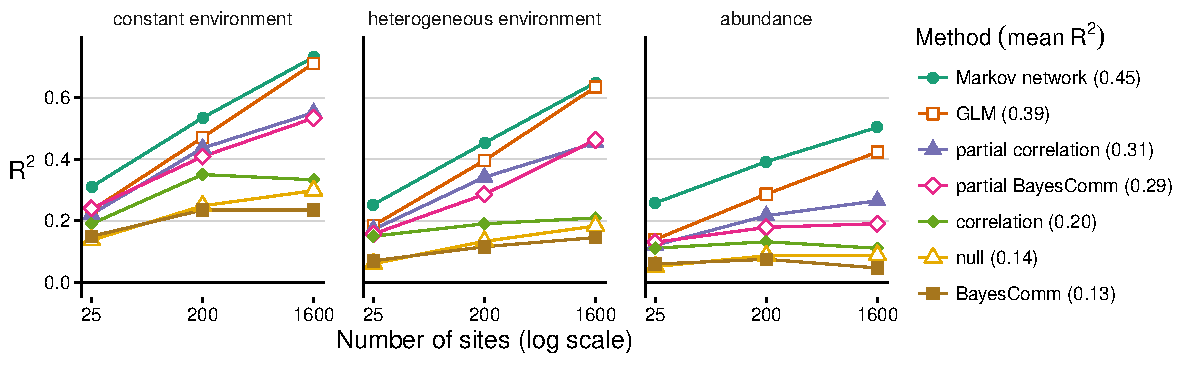
\includegraphics{manuscript-materials/figures/performance.pdf}

Summarize the results:

\begin{Shaded}
\begin{Highlighting}[]
\CommentTok{# R-squareds computed across *all* landscape types}
\NormalTok{total_ss =}\StringTok{ }\KeywordTok{mean}\NormalTok{(}\KeywordTok{resid}\NormalTok{(}\KeywordTok{lm}\NormalTok{(truth ~}\StringTok{ }\DecValTok{0}\NormalTok{, }\DataTypeTok{data =} \NormalTok{z))^}\DecValTok{2}\NormalTok{)}
\KeywordTok{round}\NormalTok{(}\DecValTok{100} \NormalTok{*}\StringTok{ }\KeywordTok{sort}\NormalTok{(}\DecValTok{1} \NormalTok{-}\StringTok{ }\KeywordTok{colMeans}\NormalTok{(resids^}\DecValTok{2}\NormalTok{) /}\StringTok{ }\NormalTok{total_ss), }\DecValTok{1}\NormalTok{)}
\end{Highlighting}
\end{Shaded}

\begin{verbatim}
##           BayesComm               Pairs         correlation 
##                11.6                15.4                18.6 
##   partial BayesComm partial correlation                 GLM 
##                26.1                27.5                29.9 
##      Markov network 
##                34.6
\end{verbatim}

\begin{Shaded}
\begin{Highlighting}[]
\CommentTok{# Rank correlations among the methods that estimate marginal relationships}
\KeywordTok{round}\NormalTok{(}\KeywordTok{cor}\NormalTok{(z[ , }\KeywordTok{c}\NormalTok{(}\DecValTok{7}\NormalTok{, }\DecValTok{10}\NormalTok{, }\DecValTok{12}\NormalTok{)], }\DataTypeTok{method =} \StringTok{"spearman"}\NormalTok{)[,}\DecValTok{1}\NormalTok{], }\DecValTok{2}\NormalTok{)}
\end{Highlighting}
\end{Shaded}

\begin{verbatim}
## correlation   BayesComm       Pairs 
##        1.00        0.85       -0.92
\end{verbatim}

Plot the true interactions versus estimated interactions for two
methods:

\begin{Shaded}
\begin{Highlighting}[]
\KeywordTok{library}\NormalTok{(ggplot2)}

\KeywordTok{ggplot}\NormalTok{(z[z$n_sites >}\DecValTok{0}\NormalTok{, ], }\KeywordTok{aes}\NormalTok{(}\DataTypeTok{x =} \StringTok{`}\DataTypeTok{Markov network}\StringTok{`}\NormalTok{, }\DataTypeTok{y =} \NormalTok{truth)) +}\StringTok{ }
\StringTok{  }\KeywordTok{stat_binhex}\NormalTok{(}\DataTypeTok{bins =} \DecValTok{100}\NormalTok{) +}\StringTok{ }
\StringTok{  }\KeywordTok{xlab}\NormalTok{(}\StringTok{"Estimated coefficient value"}\NormalTok{) +}\StringTok{ }
\StringTok{  }\KeywordTok{ylab}\NormalTok{(}\StringTok{"}\CharTok{\textbackslash{}"}\StringTok{True}\CharTok{\textbackslash{}"}\StringTok{ coefficient value"}\NormalTok{) +}\StringTok{ }
\StringTok{  }\KeywordTok{stat_hline}\NormalTok{(}\DataTypeTok{yintercept =} \DecValTok{0}\NormalTok{, }\DataTypeTok{size =} \DecValTok{1}\NormalTok{/}\DecValTok{8}\NormalTok{) +}\StringTok{ }
\StringTok{  }\KeywordTok{stat_vline}\NormalTok{(}\DataTypeTok{xintercept =} \DecValTok{0}\NormalTok{, }\DataTypeTok{size =} \DecValTok{1}\NormalTok{/}\DecValTok{8}\NormalTok{) +}\StringTok{ }
\StringTok{  }\KeywordTok{scale_fill_gradient}\NormalTok{(}\DataTypeTok{low =} \StringTok{"#F0F0F0"}\NormalTok{, }\DataTypeTok{high =} \StringTok{"darkblue"}\NormalTok{, }\DataTypeTok{trans =} \StringTok{"identity"}\NormalTok{) +}
\StringTok{  }\KeywordTok{theme_bw}\NormalTok{() +}\StringTok{ }
\StringTok{  }\KeywordTok{ggtitle}\NormalTok{(}\StringTok{"Markov network"}\NormalTok{) +}\StringTok{ }
\StringTok{  }\KeywordTok{stat_abline}\NormalTok{(}\DataTypeTok{intercept =} \DecValTok{0}\NormalTok{, }\DataTypeTok{slope =} \KeywordTok{coef}\NormalTok{(}\KeywordTok{lm}\NormalTok{(z$truth ~}\StringTok{ }\NormalTok{z$}\StringTok{`}\DataTypeTok{Markov network}\StringTok{`} \NormalTok{+}\StringTok{ }\DecValTok{0}\NormalTok{)))}
\end{Highlighting}
\end{Shaded}

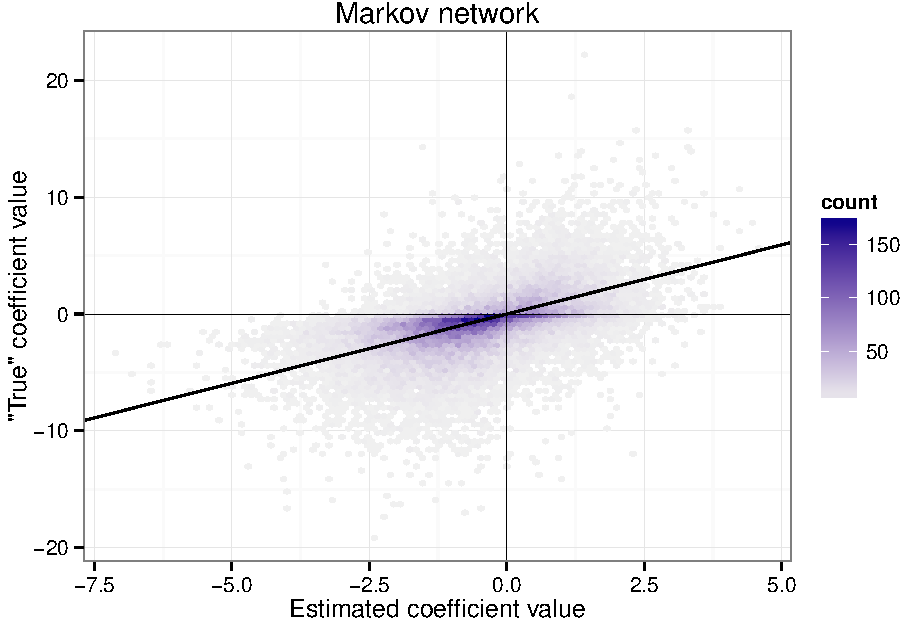
\includegraphics{recovery_files/figure-latex/unnamed-chunk-8-1.pdf}

\begin{Shaded}
\begin{Highlighting}[]
\KeywordTok{ggplot}\NormalTok{(z[z$n_sites >}\DecValTok{0}\NormalTok{, ], }\KeywordTok{aes}\NormalTok{(}\DataTypeTok{x =} \StringTok{`}\DataTypeTok{Pairs}\StringTok{`}\NormalTok{, }\DataTypeTok{y =} \NormalTok{truth)) +}\StringTok{ }
\StringTok{  }\KeywordTok{stat_binhex}\NormalTok{(}\DataTypeTok{bins =} \DecValTok{100}\NormalTok{) +}\StringTok{ }
\StringTok{  }\KeywordTok{xlab}\NormalTok{(}\StringTok{"Estimated coefficient value"}\NormalTok{) +}\StringTok{ }
\StringTok{  }\KeywordTok{ylab}\NormalTok{(}\StringTok{"}\CharTok{\textbackslash{}"}\StringTok{True}\CharTok{\textbackslash{}"}\StringTok{ coefficient value"}\NormalTok{) +}\StringTok{ }
\StringTok{  }\KeywordTok{stat_hline}\NormalTok{(}\DataTypeTok{yintercept =} \DecValTok{0}\NormalTok{, }\DataTypeTok{size =} \DecValTok{1}\NormalTok{/}\DecValTok{8}\NormalTok{) +}\StringTok{ }
\StringTok{  }\KeywordTok{stat_vline}\NormalTok{(}\DataTypeTok{xintercept =} \DecValTok{0}\NormalTok{, }\DataTypeTok{size =} \DecValTok{1}\NormalTok{/}\DecValTok{8}\NormalTok{) +}\StringTok{ }
\StringTok{  }\KeywordTok{scale_fill_gradient}\NormalTok{(}\DataTypeTok{low =} \StringTok{"#F0F0F0"}\NormalTok{, }\DataTypeTok{high =} \StringTok{"darkblue"}\NormalTok{, }\DataTypeTok{trans =} \StringTok{"identity"}\NormalTok{) +}
\StringTok{  }\KeywordTok{theme_bw}\NormalTok{() +}\StringTok{ }
\StringTok{  }\KeywordTok{ggtitle}\NormalTok{(}\StringTok{"Null model (}\CharTok{\textbackslash{}"}\StringTok{Pairs}\CharTok{\textbackslash{}"}\StringTok{)"}\NormalTok{) +}\StringTok{ }
\StringTok{  }\KeywordTok{stat_abline}\NormalTok{(}\DataTypeTok{intercept =} \DecValTok{0}\NormalTok{, }\DataTypeTok{slope =} \KeywordTok{coef}\NormalTok{(}\KeywordTok{lm}\NormalTok{(z$truth ~}\StringTok{ }\NormalTok{z$Pairs +}\StringTok{ }\DecValTok{0}\NormalTok{)))}
\end{Highlighting}
\end{Shaded}

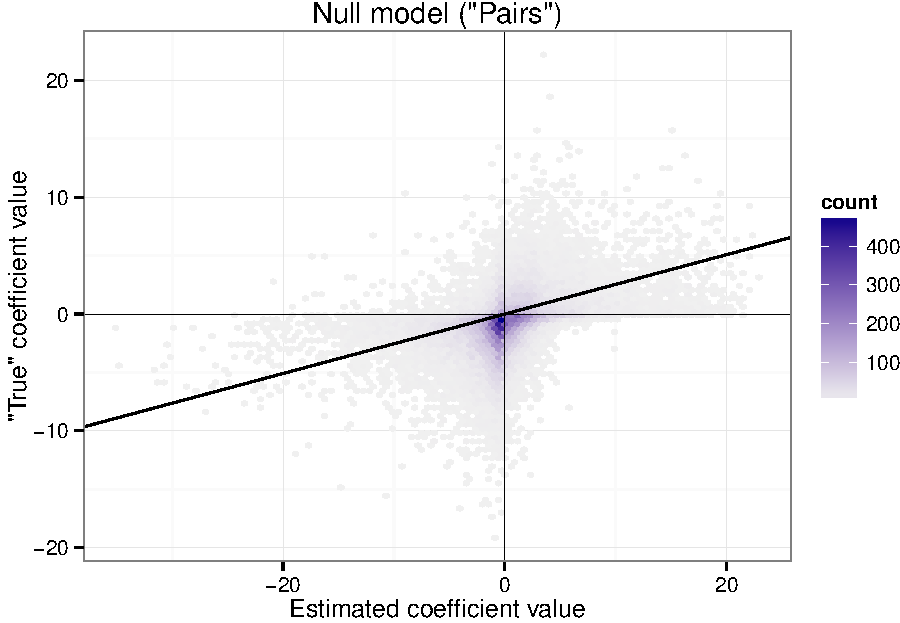
\includegraphics{recovery_files/figure-latex/unnamed-chunk-8-2.pdf}

Bootstrap resample from each of the three landscape size classes,
generating new sets of 150 landscapes. For each one, calculate the
proportion of variance explained (compared to a null baseline that
assumes all species pairs' interaction strengths are zero).

\begin{Shaded}
\begin{Highlighting}[]
\NormalTok{rep =}\StringTok{ }\DecValTok{12}
\NormalTok{n =}\StringTok{ }\DecValTok{200}
\NormalTok{boots =}\StringTok{ }\KeywordTok{replicate}\NormalTok{(}\DecValTok{500}\NormalTok{,}
          \NormalTok{\{}
            \NormalTok{boot =}\StringTok{ }\KeywordTok{lapply}\NormalTok{(}
              \NormalTok{sizes, }
              \NormalTok{function(n)\{}\KeywordTok{lapply}\NormalTok{(}
                \KeywordTok{sample.int}\NormalTok{(}\KeywordTok{max}\NormalTok{(z$rep), }\DataTypeTok{replace =} \OtherTok{TRUE}\NormalTok{),}
                \NormalTok{function(rep)\{}
                  \NormalTok{z[z$rep ==}\StringTok{ }\NormalTok{rep &}\StringTok{ }\NormalTok{z$n_sites ==}\StringTok{ }\NormalTok{n, ]}
                \NormalTok{\}}
              \NormalTok{) %>%}\StringTok{ }\NormalTok{bind_rows\}}
            \NormalTok{) %>%}\StringTok{ }\NormalTok{bind_rows}
            
            \NormalTok{resids =}\StringTok{ }\KeywordTok{sapply}\NormalTok{(}
              \KeywordTok{colnames}\NormalTok{(boot)[-(}\DecValTok{1}\NormalTok{:}\DecValTok{5}\NormalTok{)],}
              \NormalTok{function(i)\{}\KeywordTok{resid}\NormalTok{(}\KeywordTok{lm}\NormalTok{(boot$truth ~}\StringTok{ }\NormalTok{boot[[i]] +}\StringTok{ }\DecValTok{0}\NormalTok{))\}}
            \NormalTok{)}
            \NormalTok{total_ss =}\StringTok{ }\KeywordTok{mean}\NormalTok{(}\KeywordTok{resid}\NormalTok{(}\KeywordTok{lm}\NormalTok{(truth ~}\StringTok{ }\DecValTok{0}\NormalTok{, }\DataTypeTok{data =} \NormalTok{boot))^}\DecValTok{2}\NormalTok{)}
            \DecValTok{1} \NormalTok{-}\StringTok{ }\KeywordTok{colMeans}\NormalTok{(resids^}\DecValTok{2}\NormalTok{) /}\StringTok{ }\NormalTok{total_ss}
          \NormalTok{\}}
\NormalTok{)}
\end{Highlighting}
\end{Shaded}

Summarize the bootstrap results:

\begin{Shaded}
\begin{Highlighting}[]
\NormalTok{for(compared in }\KeywordTok{c}\NormalTok{(}\StringTok{"partial correlation"}\NormalTok{, }\StringTok{"correlation"}\NormalTok{, }\StringTok{"GLM"}\NormalTok{, }\StringTok{"BayesComm"}\NormalTok{, }\StringTok{"partial BayesComm"}\NormalTok{, }\StringTok{"Pairs"}\NormalTok{))\{}
  \NormalTok{CI =}\StringTok{ }\KeywordTok{round}\NormalTok{(}
    \KeywordTok{quantile}\NormalTok{(}
      \NormalTok{boots[}\StringTok{"Markov network"}\NormalTok{, ] /}\StringTok{ }\NormalTok{boots[compared, ], }
      \KeywordTok{c}\NormalTok{(.}\DecValTok{025}\NormalTok{, .}\DecValTok{975}\NormalTok{)), }
    \DecValTok{2}
  \NormalTok{)}
  
  \KeywordTok{message}\NormalTok{(}\StringTok{"R-squared is "} \NormalTok{, CI[}\DecValTok{1}\NormalTok{], }\StringTok{"-"}\NormalTok{, CI[}\DecValTok{2}\NormalTok{], }\StringTok{" times higher than from "}\NormalTok{, compared, }\StringTok{" (95% bootstrap CI)"}\NormalTok{)}
\NormalTok{\}}
\end{Highlighting}
\end{Shaded}

\begin{verbatim}
## R-squared is 1.23-1.29 times higher than from partial correlation (95% bootstrap CI)
## R-squared is 1.79-1.95 times higher than from correlation (95% bootstrap CI)
## R-squared is 1.14-1.18 times higher than from GLM (95% bootstrap CI)
## R-squared is 2.72-3.28 times higher than from BayesComm (95% bootstrap CI)
## R-squared is 1.29-1.37 times higher than from partial BayesComm (95% bootstrap CI)
## R-squared is 2.12-2.37 times higher than from Pairs (95% bootstrap CI)
\end{verbatim}

\end{document}
